\chapter{Budowa aplikacji} 
%============================================================================================================================
%							 						Glowna petla
%============================================================================================================================

\section{Główna pętla}
\lhead{Rozdział 2. \emph{Główna pętla}}

W grach komputerowych często wykorzystywane jest tzw. programowanie sterowane zdarzeniami. Polega ono na umieszczeniu w aplikacji głównej pętli, w której to cyklicznie będzie się odbywać obsługa zdarzeń (np. naciśniecie klawisza ), aktualizacja gry oraz rysowanie. Sama kolejność tych elementów nie odgrywa większej roli, warto natomiast zwrócić uwagę na to że po zatrzymaniu pętli następuje przygotowanie aplikacji do wyłączenia. W przypadku Atsro Rush po wyjściu z głównej pętli zatrzymywany jest kontekst graficzny SDL-a, zwalniane są wszystkie zajęte zasoby, i następuje wyłączenie gry. Pętla taka najczęściej implementowana jest jak while, którego zakończeniem steruje flaga wyjścia. Przy każdym obiegu pętli wartość tej flagi wyciągana jest z klasy Game, która to decyduje kiedy należy zakończyć działanie aplikacji. 

\begin{figure}[h]
    \centering
    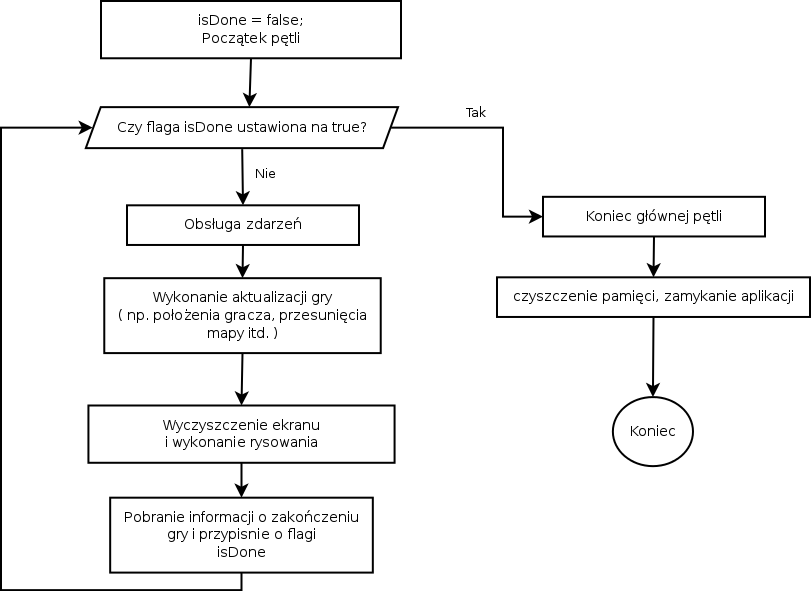
\includegraphics[width=0.8\textwidth,natwidth=410,natheight=142]{./Pictures/main_loop.png}
    \caption{Schemat działania głównej pętli}
\end{figure}

Pętla stanowi najważniejszy element większości gier, to od niej zależy czy gra będzie działać tak samo na urządzeniach różniących się wydajnością. W projekcie pętla jest dość prosta i oprócz typowych elementów typu aktualizacja, rysowanie, obsługa zdarzeń, uwzględnia jedynie sytuacje w której całość obliczeń i rysowań odbywa się zbyt szybko i należy wykonać opóźnienie. Taki problem może się pojawić na szybszych urządzeniach na których gra działała by zbyt szybko. W przypadku bardziej złożonej aplikacji można także uwzględnić sytuacje odwrotną, kiedy to ostatnia aktualizacja stanu gry odbywała się zbyt wolno i w następnym obiegu pętli należy wykonać aktualizacje kilkukrotnie żeby zapobiec braku płynności w renderowanym obrazie. Taka sytuacja jednak w grze Astro Rush nie powinna mieć miejsca z racji tego iż jest jest to gra z grafiką dwuwymiarowa i występują w niej proste obliczenia matematyczne.


%============================================================================================================================
%							 						Mapa kafelkowa
%============================================================================================================================
\section{Mapa w grze}

\lhead{Rozdział 2. \emph{Mapa kafelkowa}}
\subsection{Mapa kafelkowa}
Mapa kafelkowa (ang. tiled map) jest jedną z podstawowych technik przy tworzeniu gier z grafiką dwuwymiarową. Technika ta polega na podziale świata dostępnego w grze na fragmenty (tzw. kafelki ) o tych samych rozmiarach. Najczęściej są to kwadraty, którym przypisujemy odpowiednie identyfikatory grafik. Tak utworzona mapa przechowywana jest w postaci dwuwymiarowej macierzy w osobnym pliku na dysku, i jest wczytywana podczas startu aplikacji w osobnym wątku. Macierz składająca się wyłącznie z cyfr (typu short żeby dodatkowo oszczędzić pamięć) zajmuje o wiele mniej pamięci w przeciwieństwie do rozwiązania w którym  z dysku wczytywana jest cała mapa w postaci jednej grafiki. Na podstawie tej macierzy rysowana jest mapa widoczna na ekranie. 

Z racji tego że gracz ciągle wędruje prze mapę, ta cały czas jest przesuwana, a dokładniej  to inkrementowany jest indeks kolumny w macierzy kafelków od której zaczynamy rysowanie. Kolumna o takim indeksie rysowana jest na ekranie jako pierwsza z lewej strony, następnie rysowane są obok (po prawej stronie) kolejne kolumny aż do momentu w którym mapa pokrywa cały ekran.
Kolumna od której zaczyna się rysować od lewego brzegu ekranu przesunięta jest w lewo o pewien offset, który zwiększnay jest podczas biegu gracza do przodu. Offset ten sprawia że współrzędna na osi X skrajnej kolumny zostaje przesunięta w lewo po za ekran, tak że widoczny jest tylko fragment kolumny na ekranie. Przejście do następnej kolumny następuje w momencie kiedy skrajna kolumna znajduje się całkiem po za ekranem. Dzięki zastosowaniu takiego algorytmu nastepuje płynne przesuwanie mapy, bez widocznych przeskoków pomiędzy kolejnymi kolumnami.
 

%============================================================================================================================
%							 						Edytor leveli
%============================================================================================================================
\subsection{Edytor mapy}
\lhead{Rozdział 2. \emph{Edytor mapy}}
Opisana w poprzednim podrozdziale macierz kafelków w grze Astro Rush ma wymiary: 30000 x 15. Stąd też pojawił się problem edycji tak dużej ilości danych. Zmiana poszczególnych wpisów ręcznie nie wchodziła w grę, dlatego też powstała dodatkowa aplikacja do edycji mapy. W wizualny sposób, z wykorzystaniem jedynie myszy można w niej stworzyć w kilkanaście minut całą mapę, rozmieszczając na niej dostępne rodzaje kafelków. Edytor umożliwia także wczytanie stworzonej wcześniej mapy i jej edycje. Aplikacja została napisana z wykorzystaniem biblioteki Qt udostępnionej na licencji LGPL. Biblioteka ta jest zestawem przenośnych narzędzi do tworzenia między innymi interfejsu użytkownika, obsługi sieci, grafiki trójwymiarowej (OpenGL), plików i wielu innych. 


\begin{figure}[h]
    \centering
    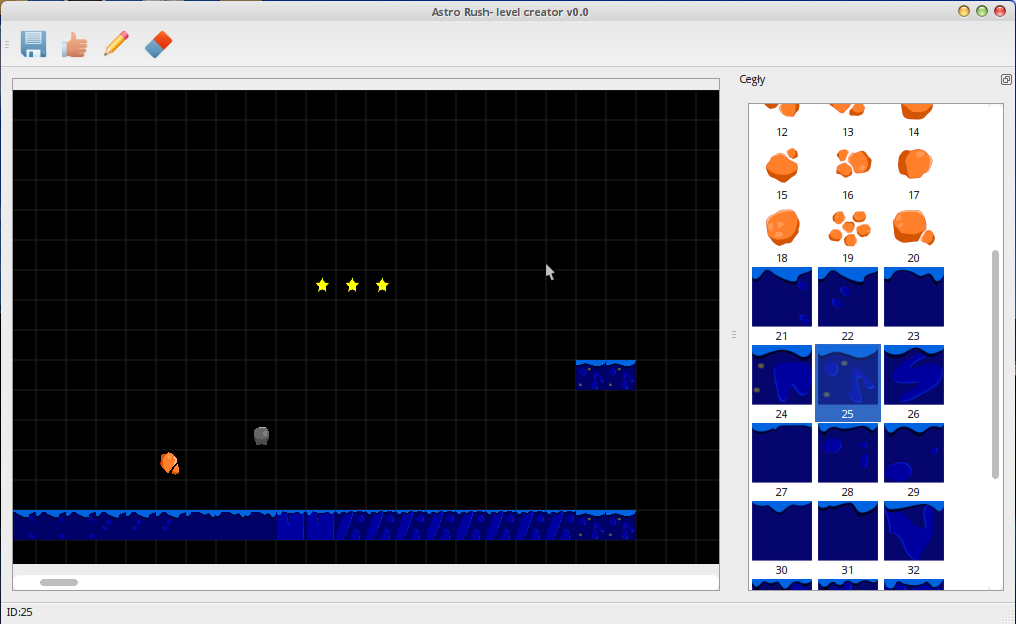
\includegraphics[width=0.8\textwidth,natwidth=800,natheight=142]{./Pictures/designer.png}
    \caption{Edytor mapy podczas pracy}
\end{figure}

Edytor mapy wyświetla całą planszę w postaci siatki na której naniesione są kafelki. Poprzez kliknięci w daną komórkę możemy zmienić rodzaj kafelka który w danym miejscu ma się wyświetlić, bądź też wyczyścić daną komórkę. Do pliku zapisywane są tylko numery odpowiadającym poszczególnym kafelkom, na bazie których gra rozpoznaje jaką grafikę w danym miejscu wstawić. Numeracja kafelków rozpoczyna się od 0, natomiast wartość -1 oznacza że w danym miejscu nie ma kafelka i taki fragment nie jest rysowany.

%============================================================================================================================
%							 						Uruchamianie aplikacji
%============================================================================================================================
\section{Uruchamianie aplikacji}
\lhead{Rozdział 2. \emph{Uruchamianie aplikacji}}
sdfd



%============================================================================================================================
%							 						Warstwy aplikacji
%============================================================================================================================
\section{Warstwy aplikacji}
\lhead{Rozdział 2. \emph{Warstwy aplikacji}}

Lorem ipsum dolor sit amet, consectetur adipiscing elit. Duis eu massa ante. Maecenas pretium metus a libero commodo convallis. Mauris a dignissim lacus. Cum sociis natoque penatibus et magnis dis parturient montes, nascetur ridiculus mus. Duis eleifend magna ut magna commodo dapibus. In adipiscing enim eget sapien elementum et adipiscing ligula sagittis. Curabitur ullamcorper cursus vulputate. Donec dignissim, tortor eget adipiscing rhoncus, risus mauris varius nisi, ac vehicula elit orci sit amet nunc. Fusce massa nisi, imperdiet vitae volutpat non, euismod ullamcorper lectus. Mauris iaculis sagittis tortor, quis convallis elit luctus eu. Sed sodales viverra velit, quis porttitor ipsum vulputate nec.








